\documentclass[12pt,a4paper]{article}

% ============================================
% PACKAGES
% ============================================
\usepackage{fontspec}
\usepackage{unicode-math}
\usepackage[vietnamese]{babel}
\usepackage{geometry}
\usepackage{graphicx}
\usepackage{amsmath}
\usepackage{listings}
\usepackage{xcolor}
\usepackage{hyperref}
\usepackage{float}
\usepackage{caption}
\usepackage{subcaption}

% ============================================
% FONT SETTINGS
% ============================================
\setmainfont{Libertinus Serif}
\setsansfont{Libertinus Sans}
\setmonofont{JetBrains Mono}[Scale=0.9]
\setmathfont{Libertinus Math}

% ============================================
% PAGE LAYOUT
% ============================================
\geometry{
    left=2.5cm,
    right=2.5cm,
    top=2.5cm,
    bottom=2.5cm
}

% ============================================
% COLORS
% ============================================
\definecolor{codegreen}{rgb}{0,0.6,0}
\definecolor{codegray}{rgb}{0.5,0.5,0.5}
\definecolor{codepurple}{rgb}{0.58,0,0.82}
\definecolor{backcolour}{rgb}{0.95,0.95,0.92}

% ============================================
% CODE LISTING STYLE
% ============================================
\lstdefinestyle{pythonstyle}{
    backgroundcolor=\color{backcolour},   
    commentstyle=\color{codegreen},
    keywordstyle=\color{blue},
    numberstyle=\tiny\color{codegray},
    stringstyle=\color{codepurple},
    basicstyle=\ttfamily\footnotesize,
    breakatwhitespace=false,         
    breaklines=true,                 
    captionpos=b,                    
    keepspaces=true,                 
    numbers=left,                    
    numbersep=5pt,                  
    showspaces=false,                
    showstringspaces=false,
    showtabs=false,                  
    tabsize=2,
    language=Python
}
\lstset{style=pythonstyle}

% ============================================
% HYPERLINK SETTINGS
% ============================================
\hypersetup{
    colorlinks=true,
    linkcolor=blue,
    filecolor=magenta,      
    urlcolor=cyan,
    pdftitle={Lab 01 - Computer Vision},
    pdfauthor={Bùi Quang Chiến},
}

% ============================================
% DOCUMENT BEGIN
% ============================================
\begin{document}

% ============================================
% TITLE PAGE
% ============================================
\begin{titlepage}
    \centering
    \vspace*{2cm}
    
    {\LARGE\bfseries TRƯỜNG ĐẠI HỌC KHOA HỌC TỰ NHIÊN\\[0.3cm]
    KHOA TOÁN - CƠ - TIN HỌC\\[0.5cm]}
    
        
    \begin{figure}[H]
    	\centering
    	\includegraphics[width=0.3\linewidth]{../../../../../LOGOHUS}
    	\label{fig:logohus}
    \end{figure}
    
    {\huge\bfseries BÁO CÁO BÀI TẬP TUẦN 1\\[0.5cm]
    MÔN: THỊ GIÁC MÁY TÍNH (MAT3562E 2)\\[0.5cm]}
    

    
    {\Large\bfseries LAB 01: XỬ LÝ ẢNH CƠ BẢN\\[0.3cm]
    HISTOGRAM VÀ POINT PROCESSING\\[1.5cm]}
    
    \begin{flushleft}
    {\large
    \textbf{Giảng viên:} TS. Cao Văn Chung\\
    \textbf{Sinh viên:} Bùi Quang Chiến\\
    \textbf{MSSV:} 23001837\\
    \textbf{Lớp:} MAT3562E 2\\
    }
    \end{flushleft}
    
    \vfill
    
    {\large Hà Nội, tháng 2 năm 2026}
\end{titlepage}

% ============================================
% TABLE OF CONTENTS
% ============================================
\tableofcontents
\newpage

% ============================================
% SECTION 1: GIỚI THIỆU
% ============================================
\section{Giới thiệu}

Bài lab này tập trung vào các kỹ thuật xử lý ảnh cơ bản trong Computer Vision, bao gồm:

\begin{itemize}
    \item Phân tích histogram và phân bố cường độ pixel
    \item Các phép biến đổi điểm ảnh (Point Processing)
    \item Kỹ thuật tăng cường chất lượng ảnh
\end{itemize}

\subsection{Mục tiêu}

\begin{enumerate}
    \item Hiểu về cấu trúc ma trận ảnh và histogram
    \item Thực hiện các phép biến đổi: Negative, Log Transform, Power Transform
    \item Áp dụng kỹ thuật Thresholding để phân đoạn ảnh
    \item So sánh hiệu quả của các phương pháp
\end{enumerate}

% ============================================
% SECTION 2: LÝ THUYẾT
% ============================================
\section{Lý thuyết cơ bản}

\subsection{Histogram}

Histogram là biểu đồ thể hiện phân bố cường độ pixel trong ảnh:
\begin{itemize}
    \item \textbf{Trục X:} Giá trị cường độ (0-255)
    \item \textbf{Trục Y:} Số lượng pixel có giá trị đó
\end{itemize}

\subsection{Point Processing}

Point Processing là phương pháp biến đổi từng pixel độc lập theo công thức:
\[ s = T(r) \]
trong đó $r$ là giá trị pixel đầu vào, $s$ là giá trị pixel đầu ra.

% ============================================
% SECTION 3: BÀI TẬP VỀ NHÀ
% ============================================
\section{Bài tập về nhà}

\subsection{Problem 1: Gray Level Modification}

\textbf{Công thức:}
\[ s = 16 \times \sqrt{r} \]

\textbf{Code Python:}
\begin{lstlisting}
def GrayLevelModification(img_input):
    f = img_input.astype(np.float32) / 255.0
    s = 16.0 * np.sqrt(f)
    s_normalized = s / s.max()
    return (255.0 * s_normalized).clip(0, 255).astype(np.uint8)
\end{lstlisting}

\textbf{Giải thích:} Hàm căn bậc hai làm sáng ảnh từ từ, hệ số 16 đảm bảo output nằm trong khoảng [0, 255].

% ============================================
\subsection{Problem 2: Median Thresholding}

\textbf{Định nghĩa:} Median $m$ thỏa mãn $P(x < m) = P(x > m)$

\textbf{Code Python:}
\begin{lstlisting}
def MedianThreshold(img_input):
    hist = cv2.calcHist([img_input], [0], None, [256], [0, 256]).ravel()
    cum_hist = np.cumsum(hist)
    total_pixels = cum_hist[-1]
    median_idx = np.searchsorted(cum_hist, total_pixels / 2.0)
    img_thresh = np.where(img_input >= median_idx, 255, 0).astype(np.uint8)
    return img_thresh, median_idx
\end{lstlisting}

\textbf{Giải thích:} Tính cumulative histogram và tìm vị trí mà tổng tích lũy bằng 50\% tổng số pixel.

% ============================================
\subsection{Problem 3: Power Transform}

\textbf{Công thức:}
\[ s = c \times r^{\gamma} \]

\textbf{Code Python:}
\begin{lstlisting}
def PowerTransform(img_input, gamma, c=1.0):
    f = img_input.astype(np.float32) / 255.0
    s = c * np.power(f, gamma)
    return (255.0 * s).clip(0, 255).astype(np.uint8)
\end{lstlisting}

\textbf{Ảnh hưởng của $\gamma$:}
\begin{itemize}
    \item $\gamma$ bé hơn 1: Làm \textbf{Sáng} ảnh hơn.
    \item $\gamma$ lớn hơn 1: Làm \textbf{Tối} ảnh đi.
    \item $\gamma$ bằng 1: Không thay đổi chất lượng hay độ sáng của ảnh.
\end{itemize}

\textbf{Kết quả thực nghiệm:}
\begin{itemize}
    \item \textbf{runway.jpg:} $\gamma = 0.7$ cho kết quả tốt nhất
    \item \textbf{spine.jpg:} $\gamma = 0.4 - 0.7$ phù hợp cho ảnh y tế
\end{itemize}

% ============================================
% SECTION 4: KẾT QUẢ
% ============================================
\section{Kết quả thực nghiệm}

\subsection{Ảnh gốc và histogram}

\begin{figure}[H]
    \centering
    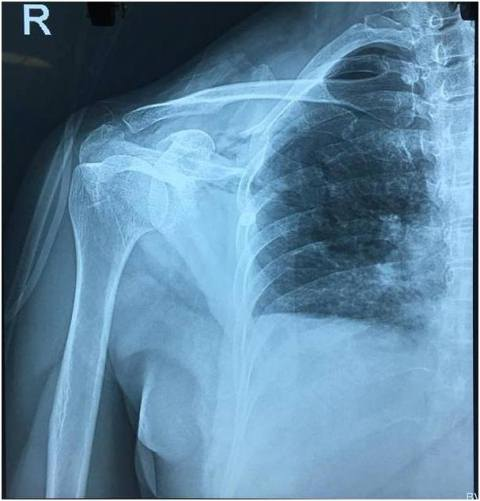
\includegraphics[width=0.8\textwidth]{Data/test_1_lab01.png}
    \caption{Kết quả các phép biến đổi trên ảnh runway.jpg}
    \label{fig:test1}
\end{figure}

\begin{figure}[H]
    \centering
    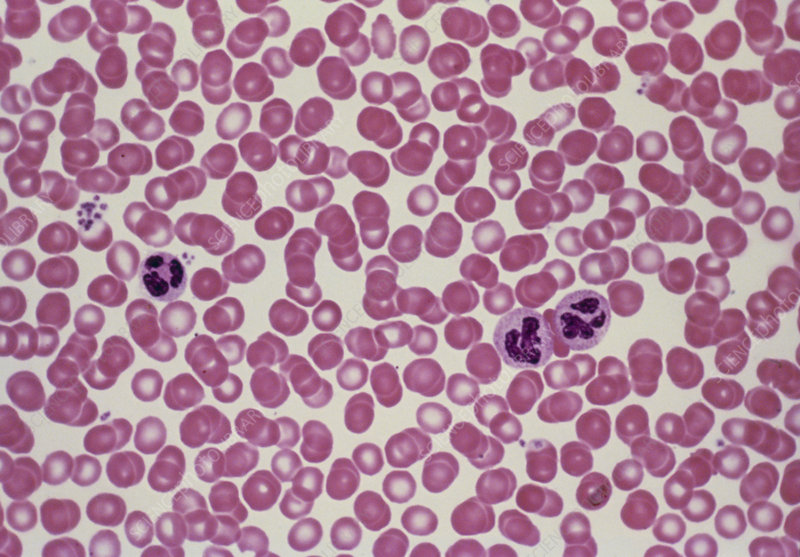
\includegraphics[width=0.8\textwidth]{Data/test_2_lab01.jpg}
    \caption{Kết quả các phép biến đổi trên ảnh spine.jpg}
    \label{fig:test2}
\end{figure}

% ============================================
% SECTION 5: SO SÁNH VÀ KẾT LUẬN
% ============================================
\section{So sánh và kết luận}

\subsection{So sánh các phương pháp}

\begin{table}[H]
\centering
\caption{So sánh các phương pháp xử lý ảnh}
\begin{tabular}{|l|p{4cm}|p{4cm}|}
\hline
\textbf{Phương pháp} & \textbf{Ưu điểm} & \textbf{Nhược điểm} \\
\hline
Gray Level Mod & Đơn giản, luôn làm sáng & Không linh hoạt \\
\hline
Median Threshold & Phân đoạn nhanh & Mất thông tin \\
\hline
\textbf{Power Transform} & \textbf{Linh hoạt nhất} & Cần chọn $\gamma$ \\
\hline
\end{tabular}
\end{table}

\subsection{Kết luận}

\begin{itemize}
    \item \textbf{Power Transform là phương pháp tốt nhất} vì có thể điều chỉnh $\gamma$ phù hợp với từng loại ảnh
    \item Ảnh y tế (spine): Dùng $\gamma = 0.4 - 0.7$
    \item Ảnh tự nhiên (runway): Dùng $\gamma = 0.7$
    \item Histogram giúp phân tích phân bố cường độ pixel hiệu quả
\end{itemize}

% ============================================
% REFERENCES
% ============================================
\section{Tài liệu tham khảo}

\begin{enumerate}
    \item OpenCV Documentation: \url{https://docs.opencv.org/}
    \item NumPy Documentation: \url{https://numpy.org/doc/}
\end{enumerate}

\end{document}
